% !TeX root = main.tex

% ============================================================
% thesis-sync entry: 2026-07-06_pneumatic-coupling-connector
% Type: design decision + theoretical idea + experimental observation
% Insertable section block (no preamble). Requires: graphicx, amsmath.
% Figure \includegraphics lines are COMMENTED so the file compiles standalone.
% ============================================================

\section{PNEUMATIC COUPLING OF BODY AND TAIL}
\label{sec:lizard-connector}

\subsection{Central Connector and Channel Routing}

The body and tail segments are joined by a rigid central connector that
performs three functions: it mechanically couples the two segments, it
routes their internal chambers pneumatically, and it carries the external
pressure inlet. The connector contains internal channels of less than
1~mm diameter that link chambers of the body segment to chambers of the
tail segment. Two routing topologies are implemented within the same
connector. In the \emph{crossed} routing, an internal channel connects a
chamber of the body to a chamber on the opposite side of the tail, so
that a single pressure input inflates chambers lying on opposite sides of
the body--tail axis; the two segments then bend with opposite curvature
signs, and the unit assumes an S-shaped centerline. In the
\emph{uncrossed} routing, the channel connects chambers lying on the same
side of both segments, so that both segments bend with the same curvature
sign and the unit assumes a U-shaped centerline. The deformation mode of
the coupled unit is therefore selected purely by the choice of the
addressed chamber pair, without any additional valve or actuator at the
joint.

\subsection{Inlet Asymmetry and Effective Pressure Transmission}

The pressure inlet is located asymmetrically with respect to the two
segments, closer to the body side. Because the two segments communicate
only through the narrow ($<$1~mm) connector channels, the segment closer
to the inlet receives the supply pressure more directly, whereas the
distal segment is fed through the additional flow resistance of the
channel. At quasi-static equilibrium, the body segment is observed to
bend more than the tail segment under a shared input. For modeling
purposes, this asymmetry is abstracted as an effective pressure
transmission ratio
\begin{equation}
  P_t = \alpha \, P_b, \qquad 0 < \alpha \leq 1,
  \label{eqn:lizard-alpha}
\end{equation}
where $P_b$ is the effective pressure acting in the body segment, $P_t$
the effective pressure acting in the tail segment, and $\alpha$ an
experimentally identified transmission ratio. It should be emphasized
that (\ref{eqn:lizard-alpha}) is a lumped abstraction: the internal
pressures of the two segments have not been measured independently, and
the attribution of the bending asymmetry to viscous losses in the narrow
channel, while plausible, has not been verified with dedicated pressure
sensing in both segments. The safe claim supported by the present
hardware is that the inlet placement and the narrow connecting channels
produce an asymmetric effective actuation of the two segments.

\subsection{Demonstrated Deformation Modes}

Both deformation modes were demonstrated on the bare coupled actuator and
on the assembled robot. On the assembled robot, horizontal S-shaped
bending of the body--tail axis was obtained at input pressures of
approximately 10--11~kPa, with each segment reaching a bending angle of
approximately 75$^{\circ}$ at 11~kPa. Vertical U-shaped bending, in which
the coupled unit lifts against gravity while the posterior suction-cup
feet remain attached to the substrate, was obtained in the same pressure
range (10.5--11.4~kPa, including tip-loaded cases reported in
Section~\ref{sec:lizard-ubend-loads}). The input pressure was recorded in
every experiment frame by including the digital pressure display (PPX
series, CKD) in the camera field of view, so that pressure and
deformation can be correlated during image-based analysis.

% --- Figures (paths to be fixed by the author; commented for compilation) ---
\begin{figure}[tb]
  \centering
  % 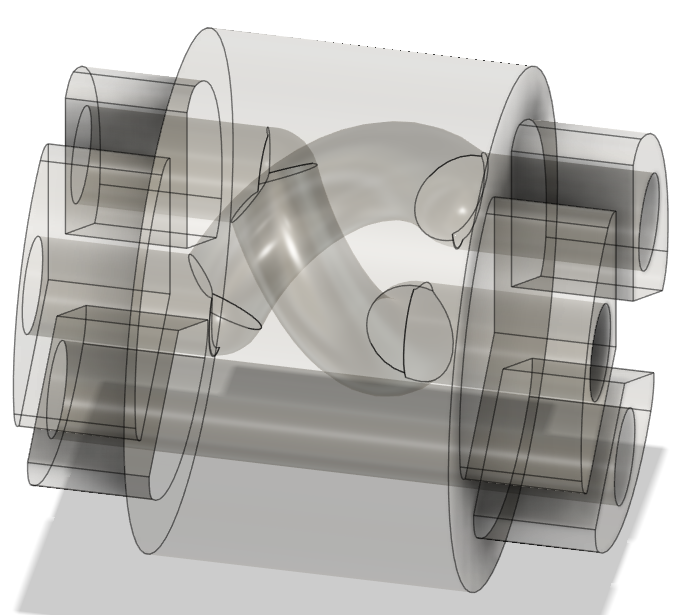
\includegraphics[height=38mm]{figures/bodytailconnector.png}
  % 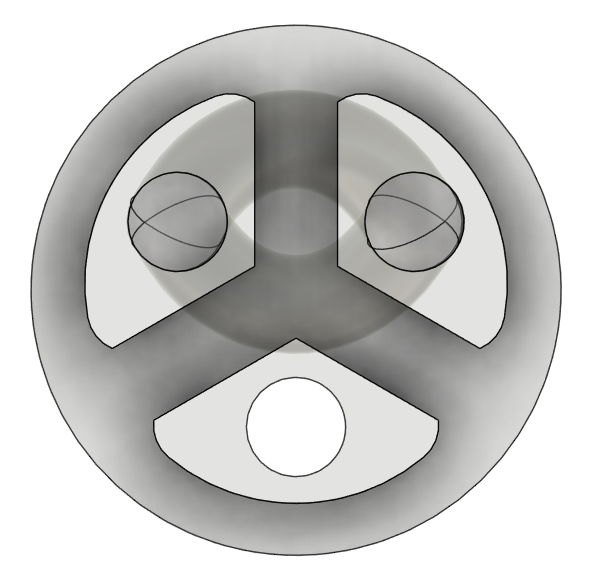
\includegraphics[height=38mm]{figures/bodytailconnectorsection.png}
  \caption{Central body--tail connector. (a)~Transparent CAD view showing
  the internal channel routing between the chamber interfaces of the two
  segments. (b)~Cross-sectional view showing the three 120$^{\circ}$
  chamber interfaces and the sub-millimeter internal channels.}
  \label{fig:lizard-connector}
\end{figure}

\begin{figure}[tb]
  \centering
  % 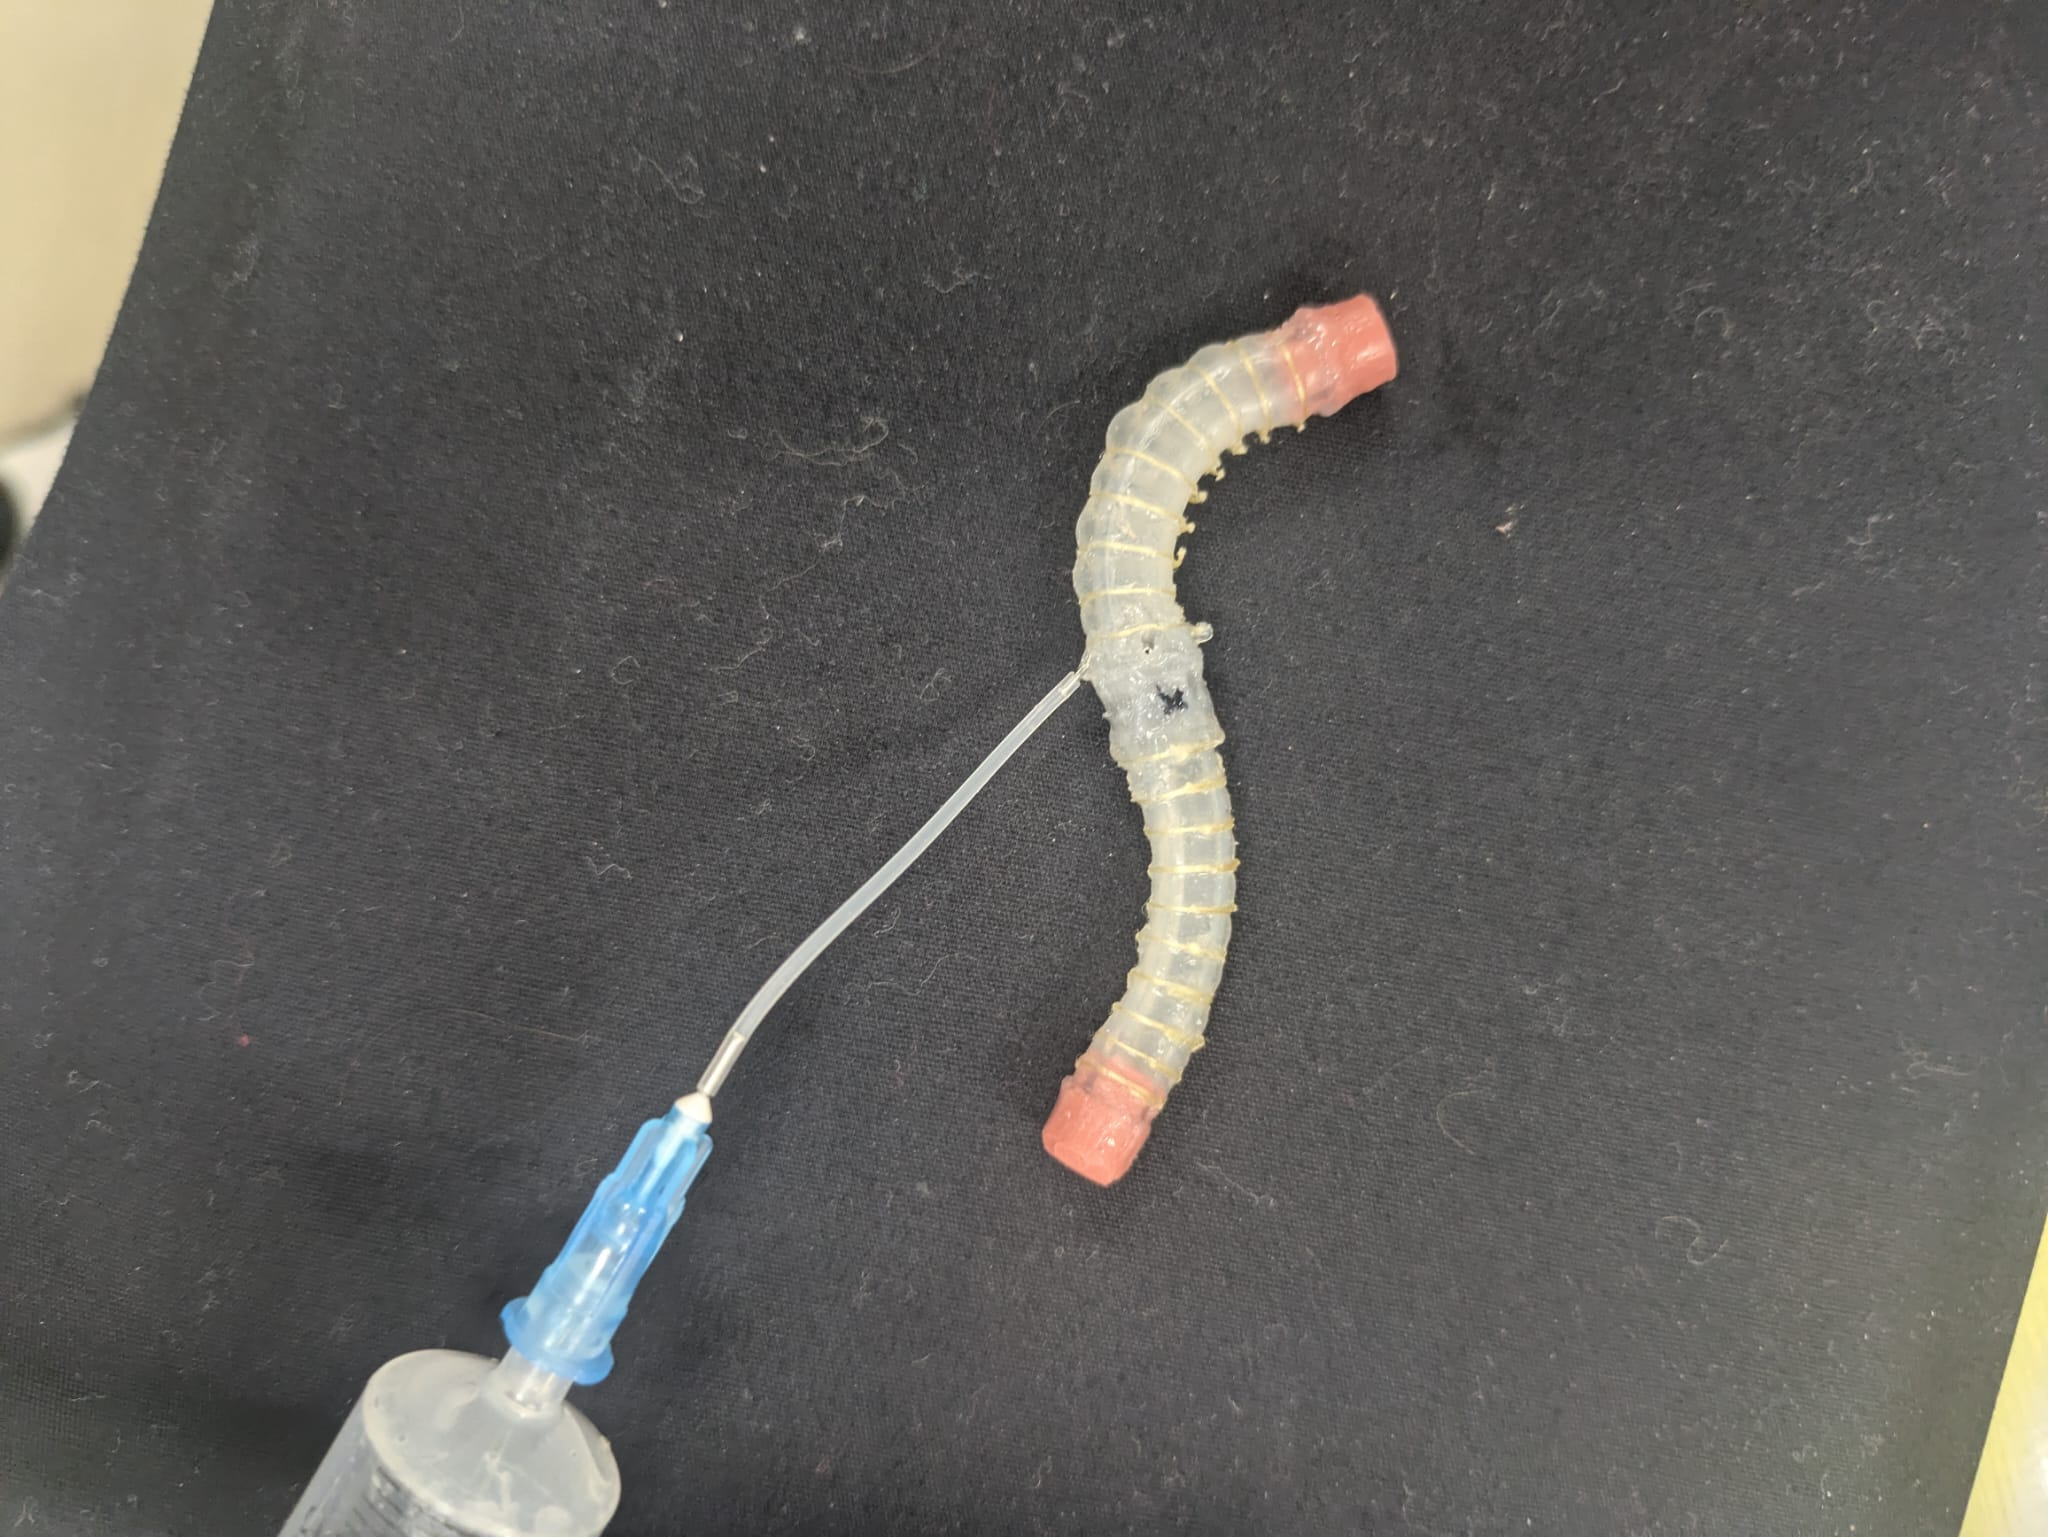
\includegraphics[height=38mm]{figures/lizardBodyS.jpeg}
  % 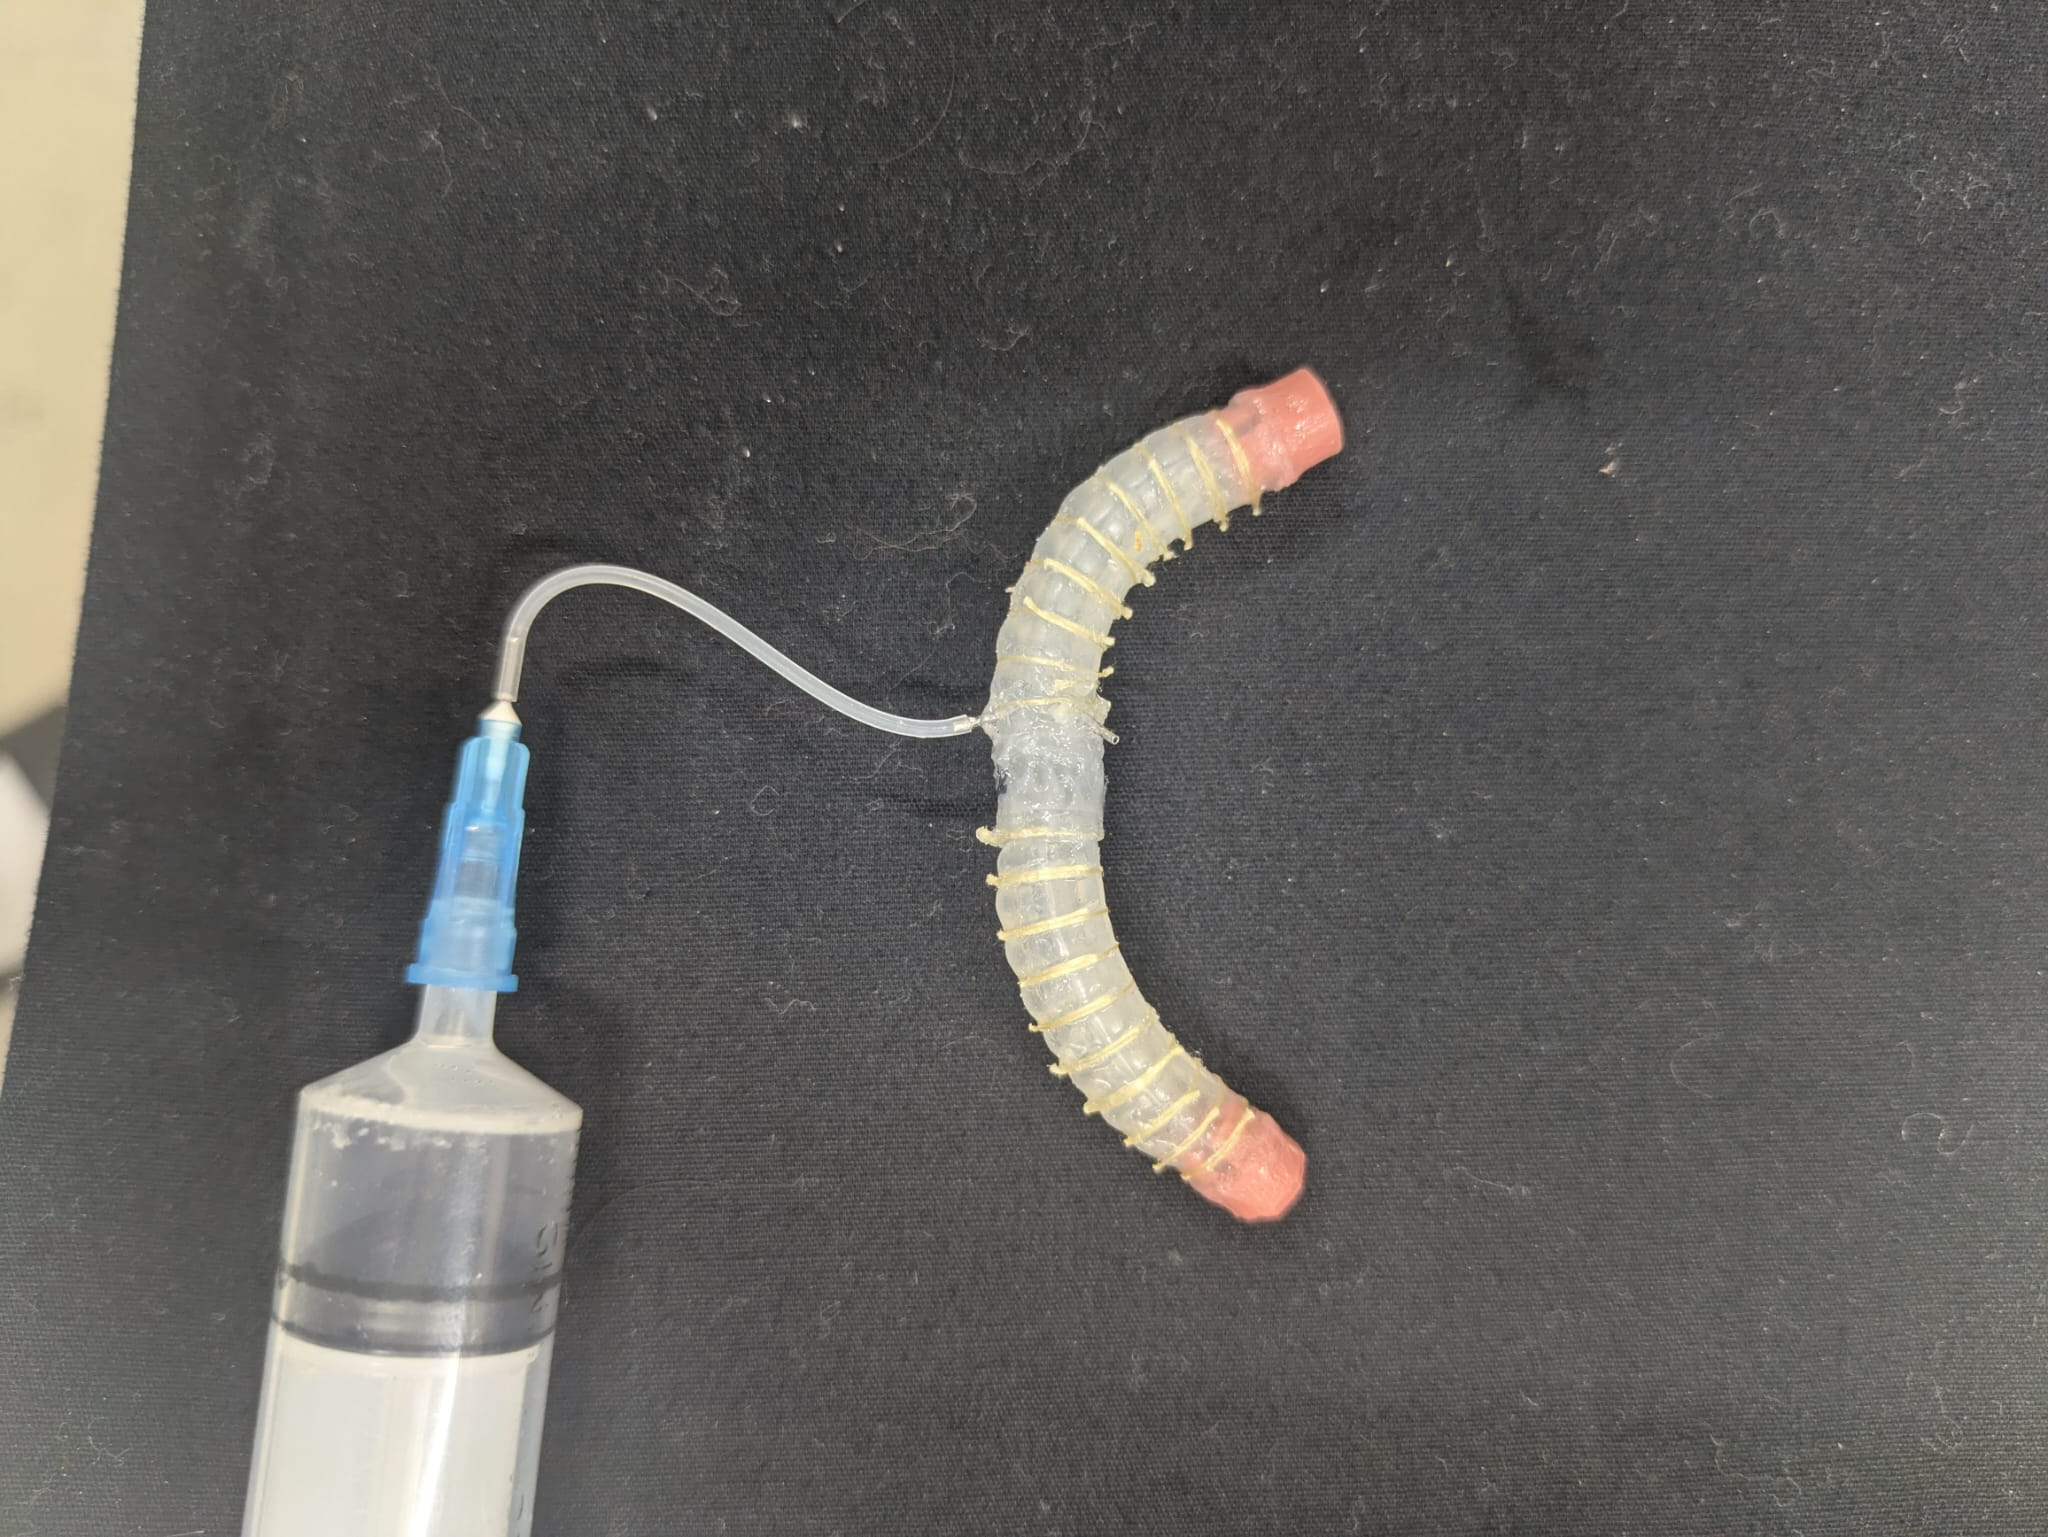
\includegraphics[height=38mm]{figures/lizardBodyU.jpeg}
  \caption{Deformation modes of the bare coupled body--tail actuator under
  a single manually applied pressure input. (a)~S-shaped bending through
  the crossed chamber path. (b)~U-shaped bending through the uncrossed
  chamber path.}
  \label{fig:lizard-s-u-modes}
\end{figure}
